%%%%%%%%%%%%%%%%%%%%%%%%%%%%%%%%%%%%%%%%%%%%%%
%                insertmeeting
% 1) Title (something creative & funny?)
% 2) Date (MM/DD/YYYY)
% 3) Location (ex. Hagerty High School)
% 4) People/Committees Present 
% 5) Picture 
% 6) Start Time & Stop Time (ex. 12:30AM to 4:30PM)
%%%%%%%%%%%%%%%%%%%%%%%%%%%%%%%%%%%%%%%%%%%%%%
\insertmeeting 
	{Meeting Example} 
	{09/18/21}
	{Hagerty High School}
	{Jensen}
	{Images/RobotPics/robot.jpg}
	{10:00 - 3:30}
	
\subsection*{Hardware}
\noindent\hfil\rule{\textwidth}{.4pt}\hfil
\subsubsection*{Goals}
\begin{itemize}
    \item Design a grabber for intake
    \item Finish constructing car drivetrain  

\end{itemize} 

\noindent\hfil\rule{\textwidth}{.4pt}\hfil

\subsubsection*{Accomplishments}
Today, we once again met at UCF and continued working on hardware. At the beginning of the meeting, we decided to split up into teams and work in parallel on different parts of the robot. Some of us went to continue working on the front wheel of the car drivetrain, while others started working on the intake for the tank drive robot. 
The drivetrain committee started off quickly, building the front wheel assembly as we had designed it in CAD. While we were working, we realized that we had forgotten to print the ramp that angles the front wheel. Because we didn’t want to have to wait too long to continue working on the drivetrain, we decided to make a new sloped part that we can laser cut. Because the laser cutter can cut parts much quicker than a 3d printer, we were able to quickly design the laser cut slope part in CAD (Figure \ref{fig:pic1}) then cut it out fairly quickly. Once off the laser cutter, we glued all of the sides of the part together then screwed it onto our rev extrusions (Figure \ref{fig:pic2}). From there, we were able to attach the front wheel onto the drivetrain, completing it for the time being.
Over in the intake committee, we started working on a simple grabber that could be attached to the arm. This paired with the spatula part we built at a previous meeting will clamp and hold a block so we can lift it up and into a goal. We started off in CAD, recreating the arm in cad (Figure \ref{fig:pic3}). With the arm created, we began making sketches of  a “finger” piece that can attach to a servo. Referring to our sketch, we created the finger part in CAD. At the end of the finger piece is another plate which we plan to attach rubber to the end of to give it a better grip (Figure \ref{fig:pic4}). We quickly laser cut the finger parts and attached them onto the robot (Figure \ref{fig:pic5}).
One issue that we have run into in the past with arm mechanisms similar to what we have this year is that the PID algorithm is too slow to accurately hold it up. This means that when placing cargo into the shipping hubs the arm will wobble and will be generally inaccurate. To remedy this, we came up with a hardware solution to a software problem by creating a back stop for the arm where the arm can just slam into a plate at a predetermined height that holds it at the right angle to drop cargo into a level of the shipping hub. At the moment, the back stop will stop the arm at the height of the middle goal, but in the future, we want to have a variable-height backstop that will hold the arm at predetermined heights for each of the levels of the shipping hub. For now, we made a CAD design for the mid level back stop, cut it out, then attached it to the back of the robot (Figure \ref{fig:pic6}).

 

\begin{figure}[ht]
\centering
\begin{minipage}[b]{.50\textwidth}
  \centering
  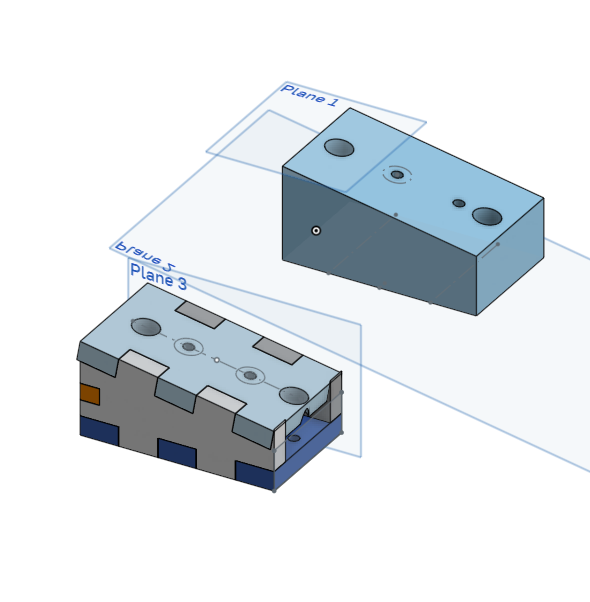
\includegraphics[width=0.8\textwidth]{Meetings/October/10-11-21/10-11-21_Hardware_Figure1 - Nathan Forrer.PNG}
  \caption{The wheel ramps.}
  \label{fig:pic1}
\end{minipage}%
\hfill%
\begin{minipage}[b]{.50\textwidth}
  \centering
  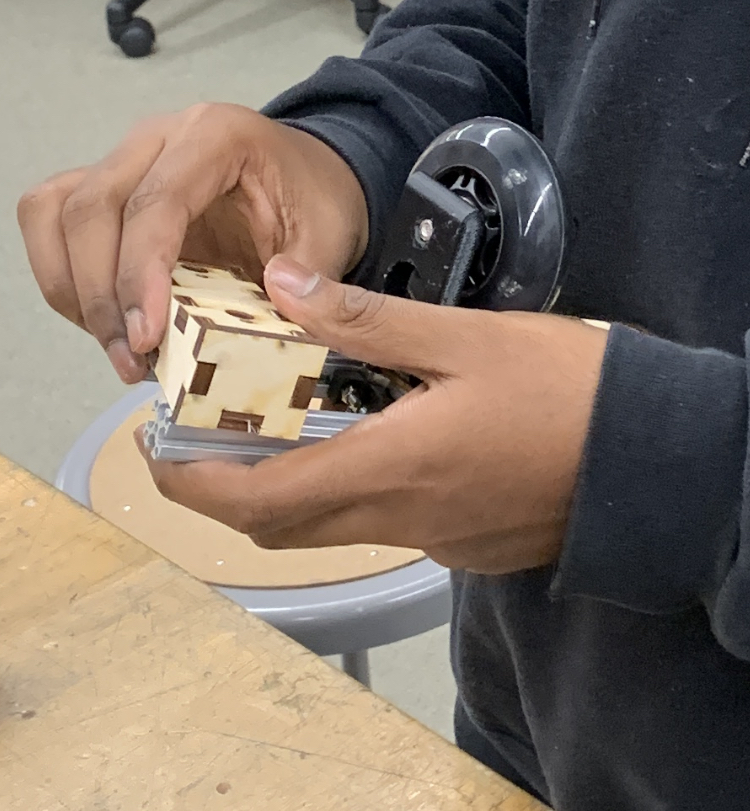
\includegraphics[width=0.8\textwidth]{Meetings/October/10-11-21/10-11-21_Hardware_Figure2 - Nathan Forrer.jpg}
  \caption{Assembling the front wheel.}
  \label{fig:pic2}
\end{minipage}
\end{figure}

\begin{figure}[ht]
\centering
\begin{minipage}[b]{.50\textwidth}
  \centering
  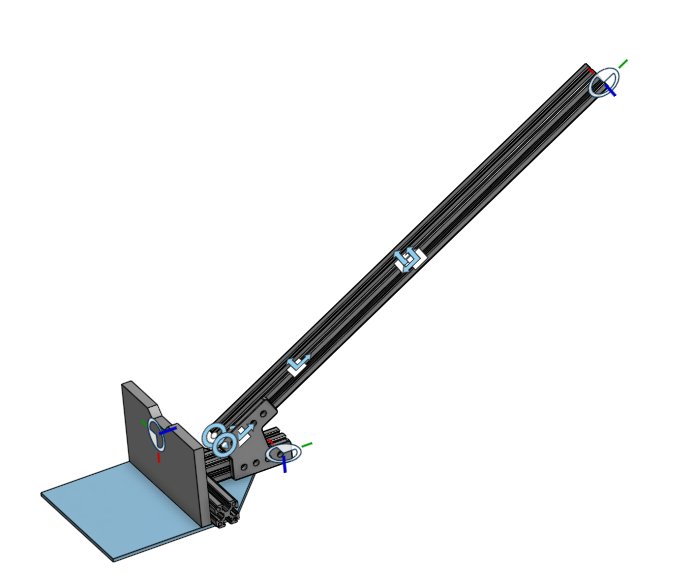
\includegraphics[width=0.8\textwidth]{Meetings/October/10-11-21/10-11-21_Hardware_Figure3 - Nathan Forrer.PNG}
  \caption{The arm CAD file.}
  \label{fig:pic3}
\end{minipage}%
\hfill%
\begin{minipage}[b]{.50\textwidth}
  \centering
  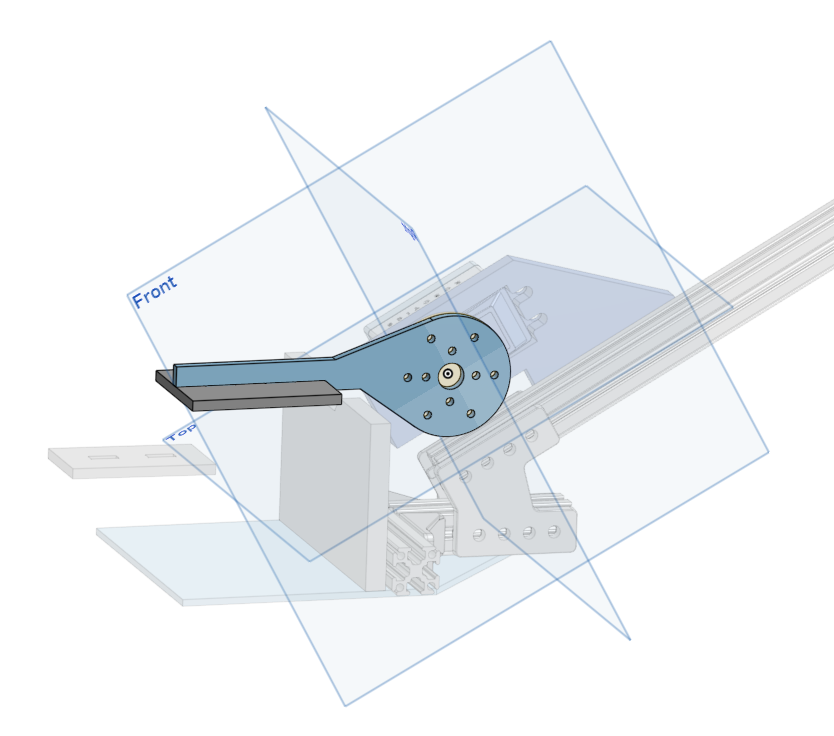
\includegraphics[width=0.8\textwidth]{Meetings/October/10-11-21/10-11-21_Hardware_Figure4 - Nathan Forrer.PNG}
  \caption{Grabber design.}
  \label{fig:pic4}
\end{minipage}
\end{figure}

\begin{figure}[ht]
\centering
\begin{minipage}[b]{.50\textwidth}
  \centering
  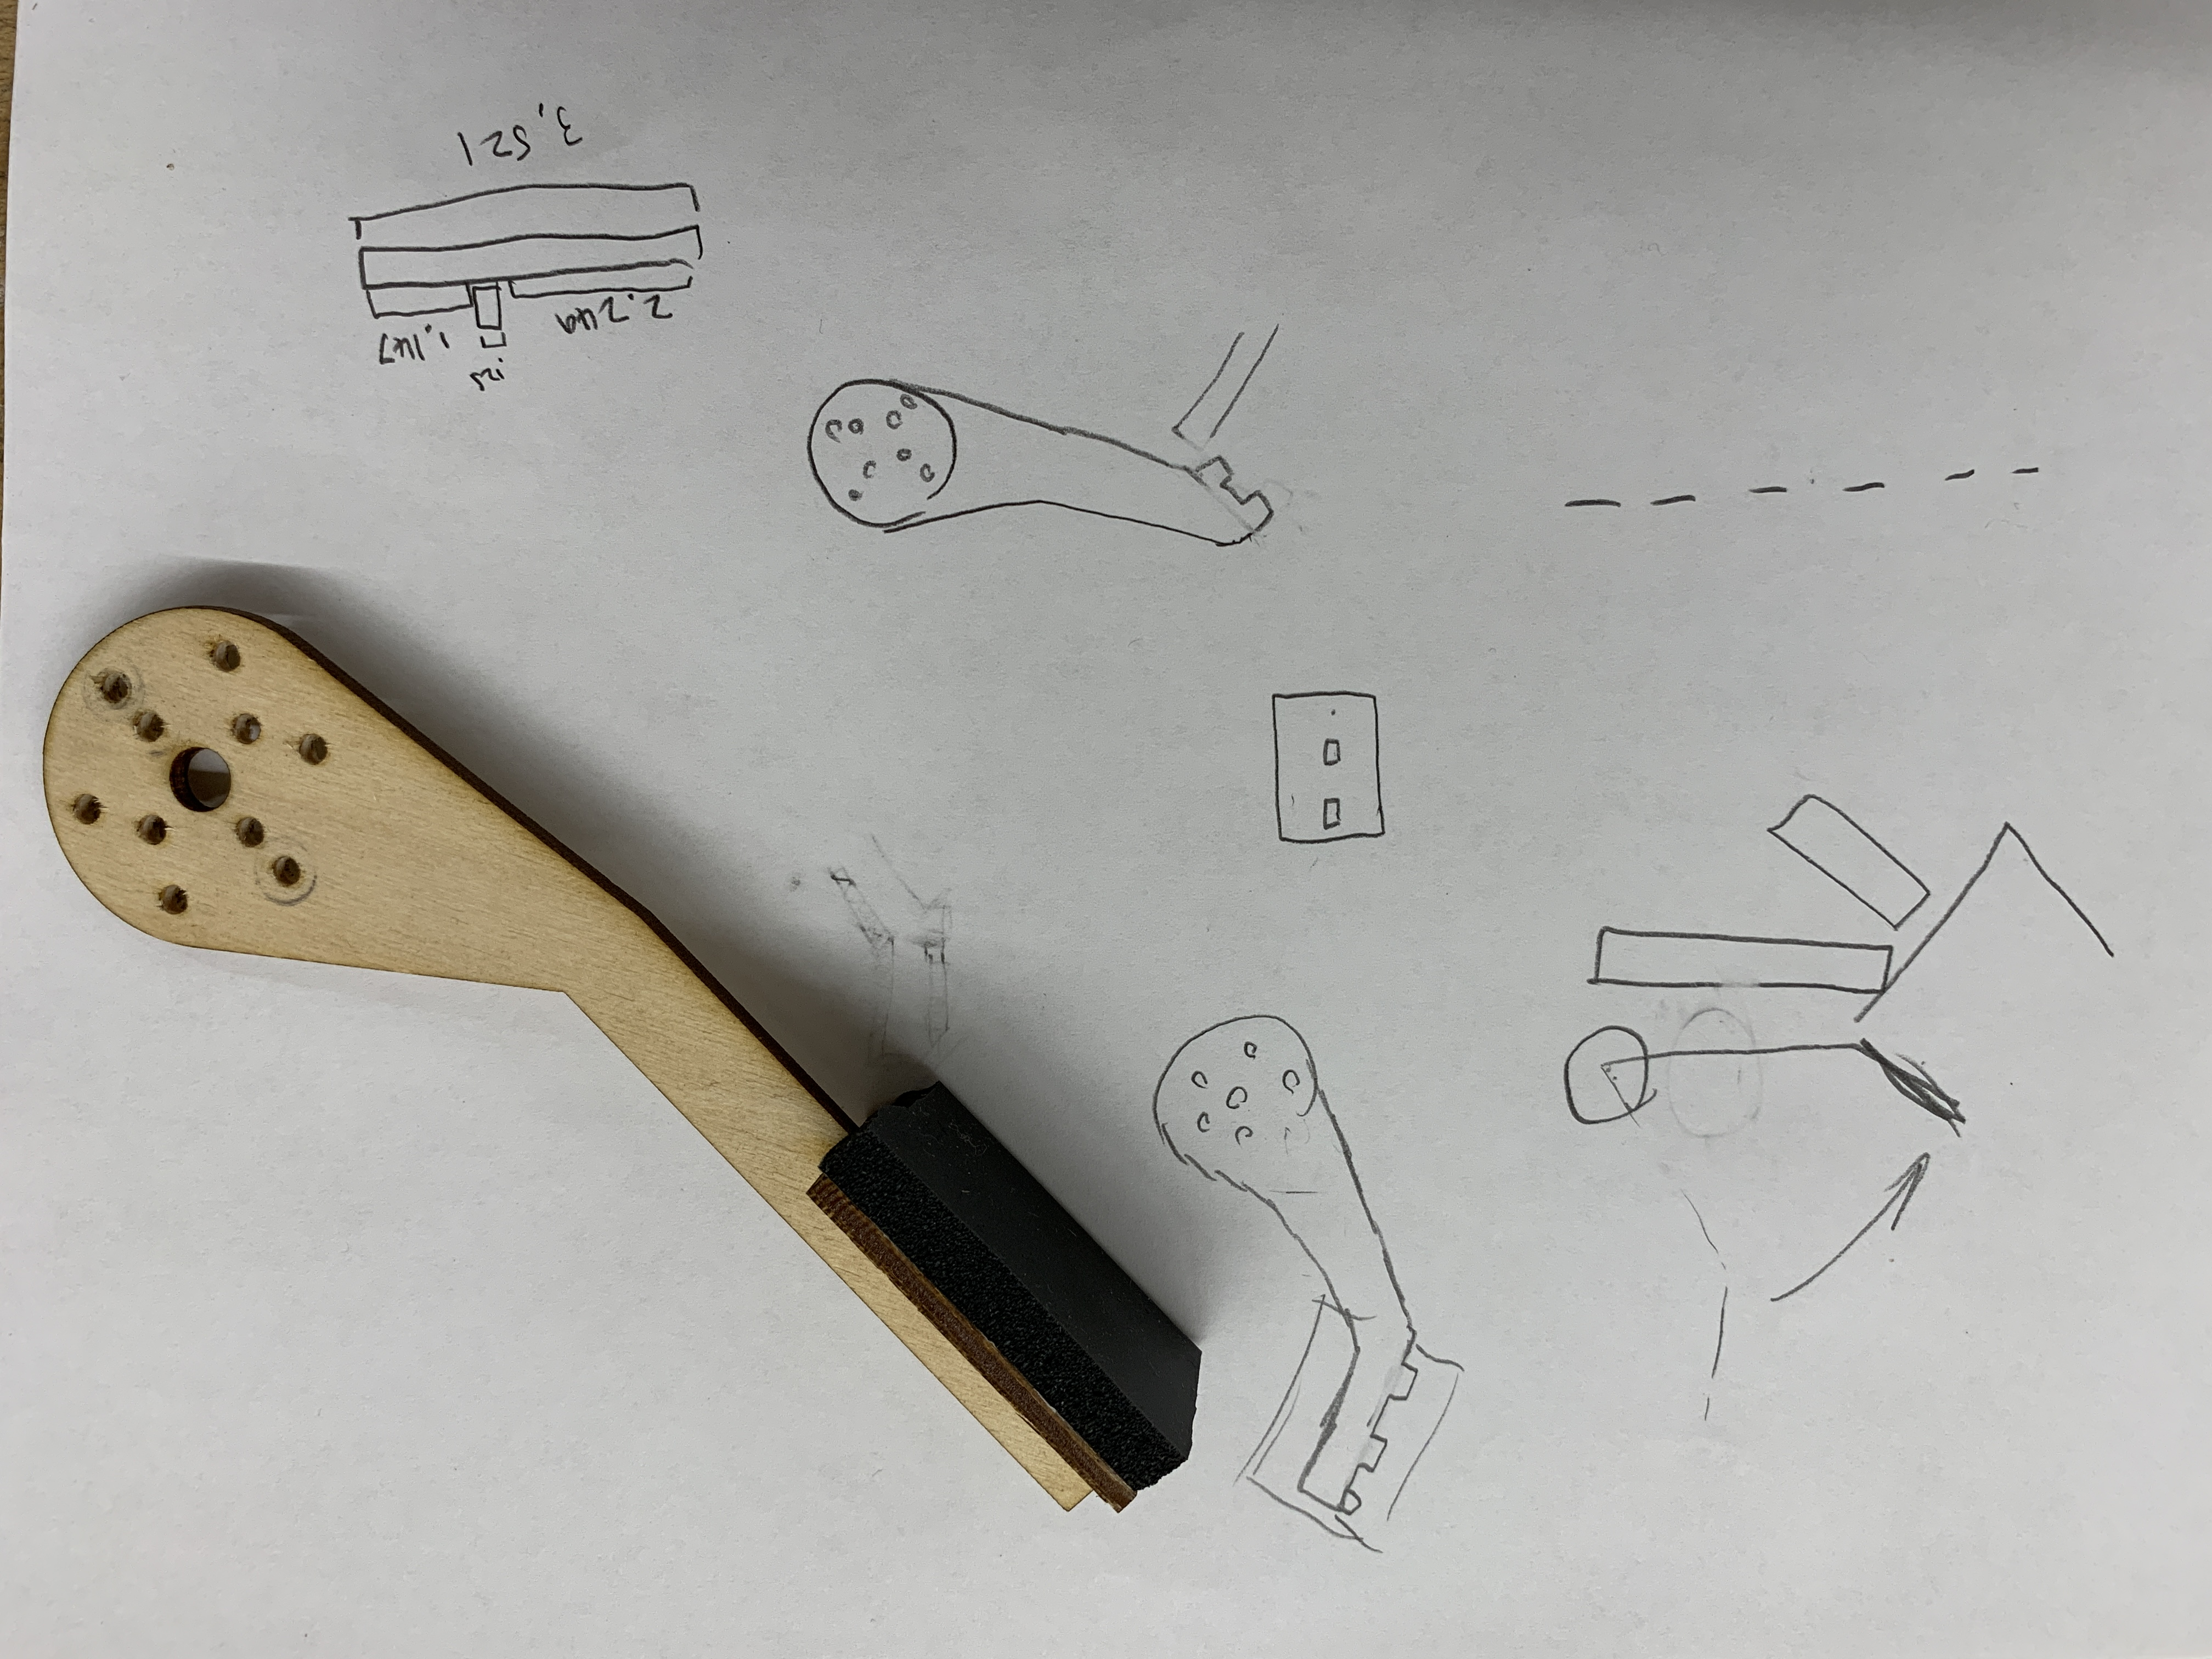
\includegraphics[width=0.8\textwidth]{Meetings/October/10-11-21/10-11-21_Hardware_Figure5 - Nathan Forrer.JPG}
  \caption{Our assembled grabbar and sketches.}
  \label{fig:pic5}
\end{minipage}%
\hfill%
\begin{minipage}[b]{.50\textwidth}
  \centering
  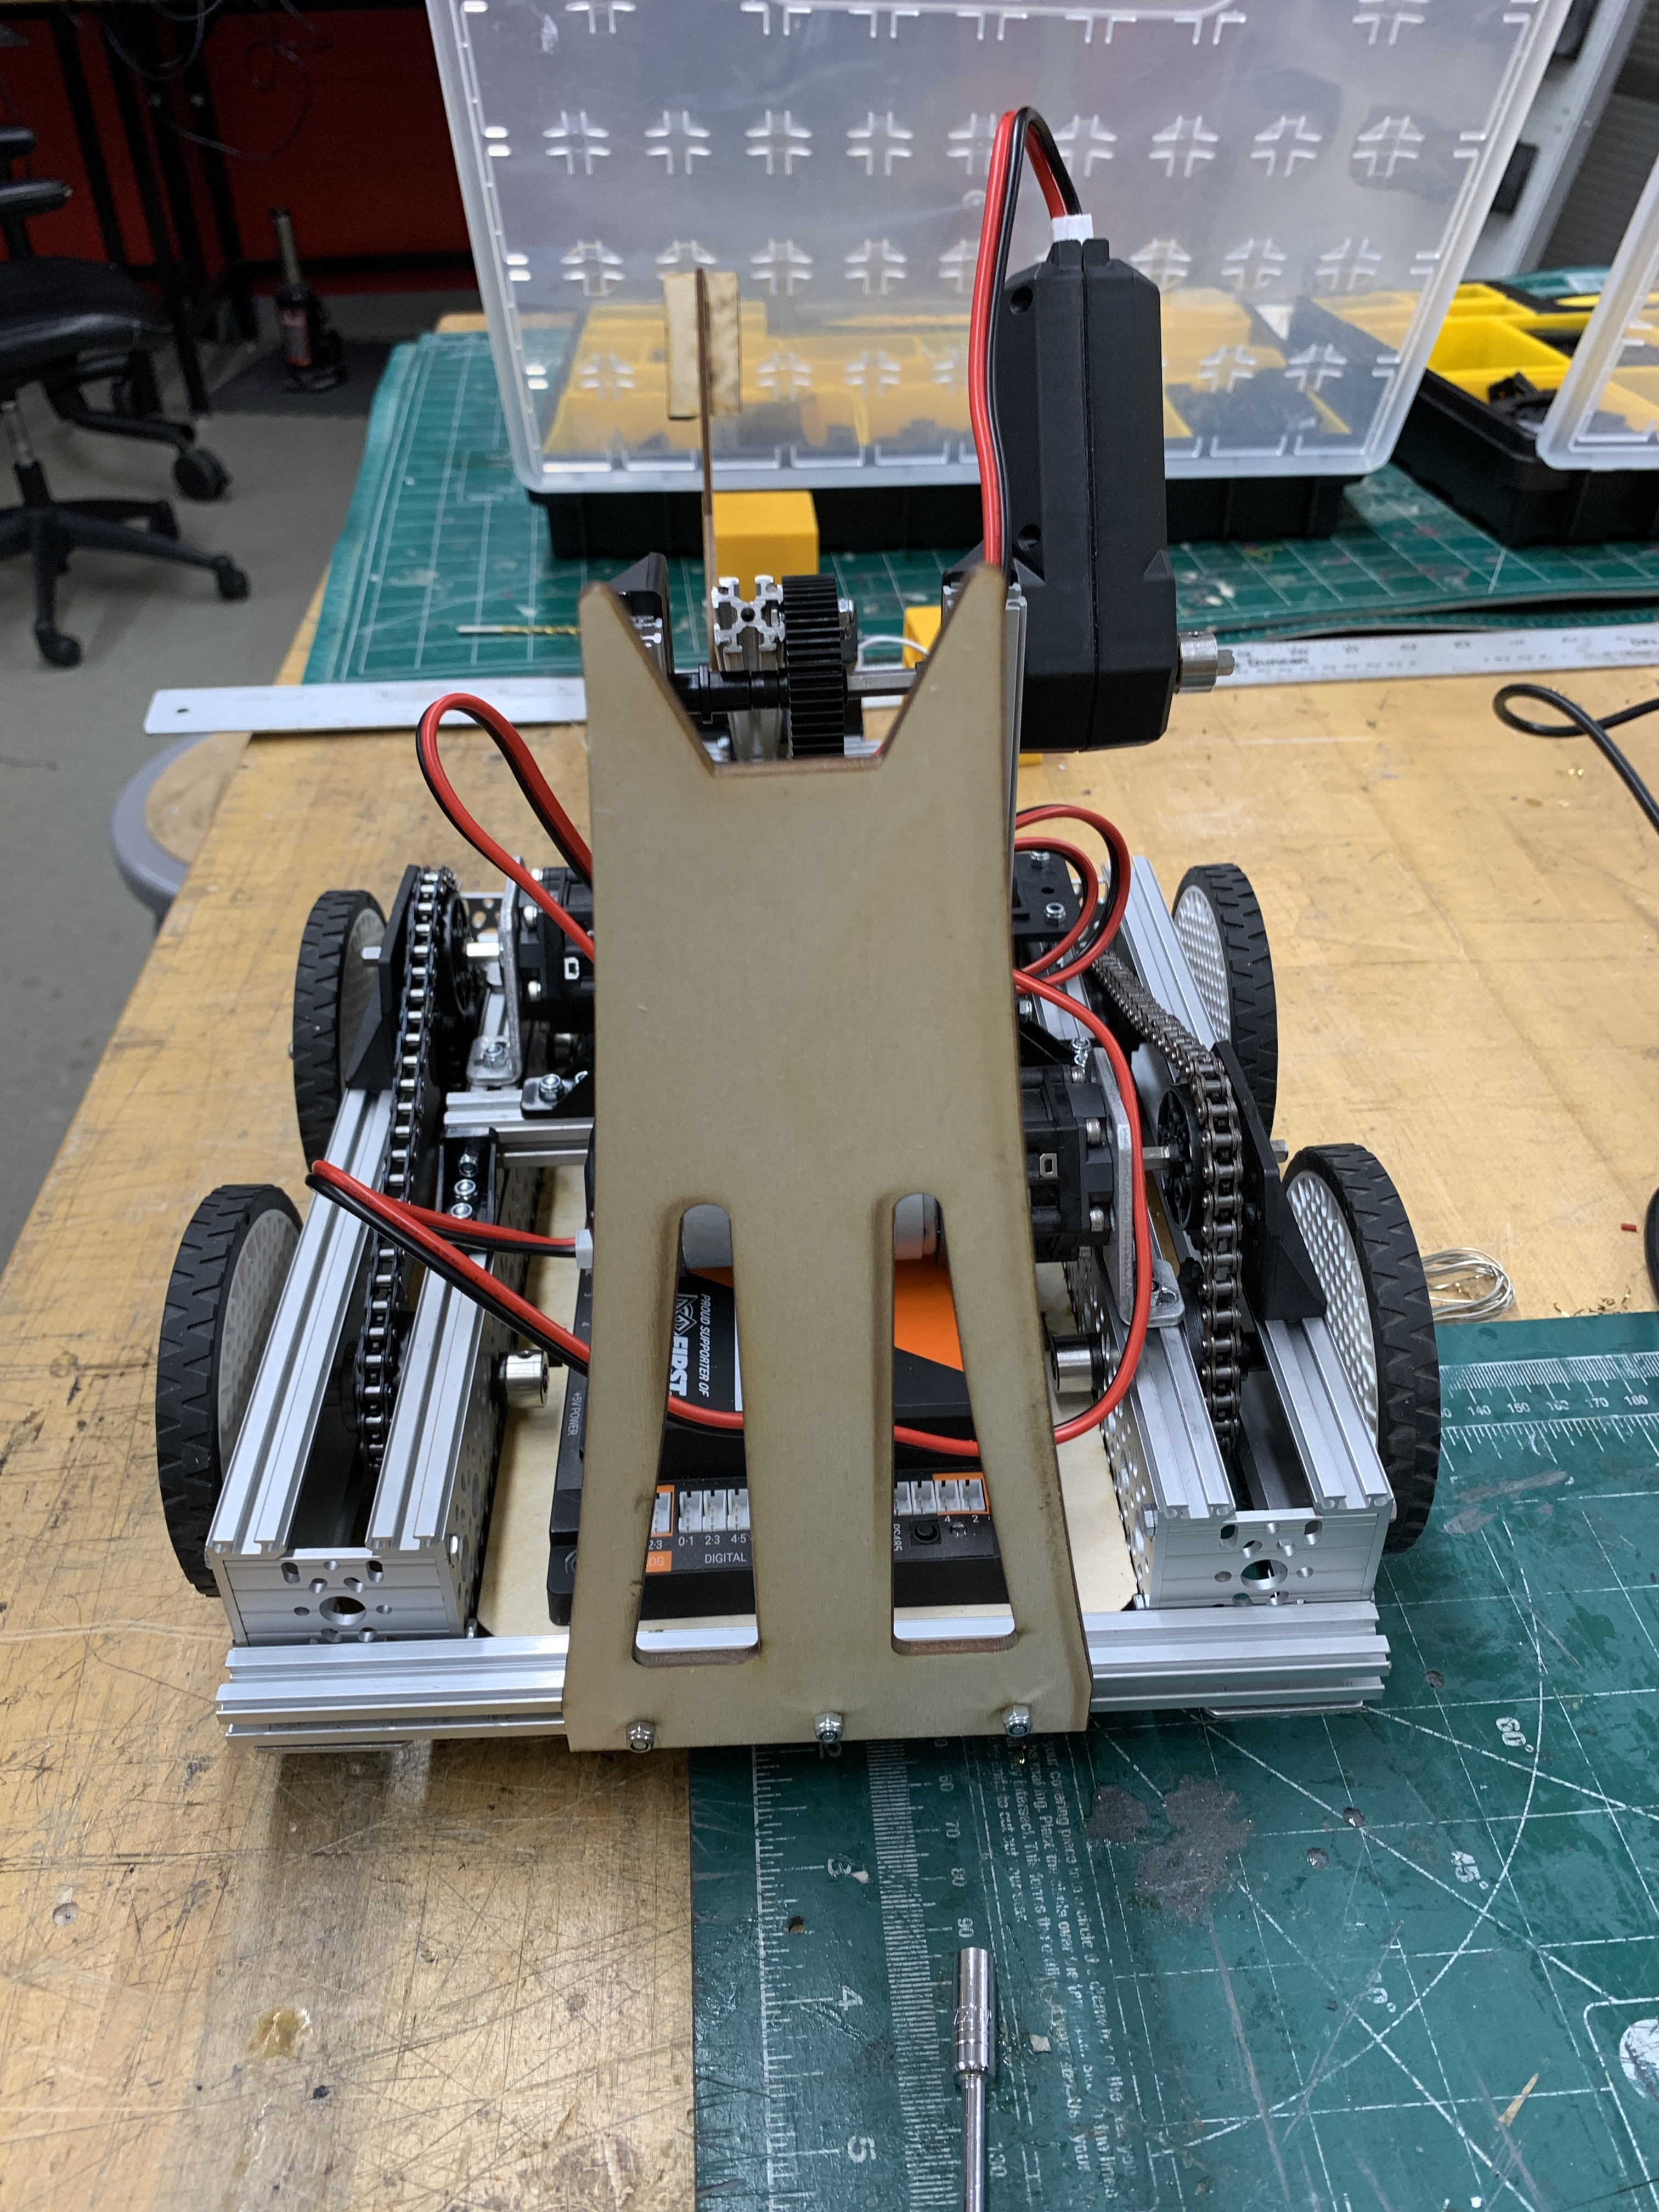
\includegraphics[width=0.8\textwidth]{Meetings/October/10-11-21/10-11-21_Hardware_Figure6 - Nathan Forrer.JPG}
  \caption{The assembled back stop.}
  \label{fig:pic6}
\end{minipage}
\end{figure}


